\section{Minimum cut problem}

Let $G = (V, E)$ be a connected, undirected graph, where $n = |V|$ and $m = |E|$ represent the number of vertices and edges, respectively. 
For any subset $S \subset V$, the set $\delta(S) = \{(u, v) \in E : u \in S, v \in S^\prime\}$ represents a cut. 
The goal of the minimum cut problem is to find the cut with the fewest number of edges.

\paragraph*{Source-target cut problem}
In graph theory, a source-target cut refers to a way of partitioning the vertices of a graph into two disjoint subsets such that: one subset contains a designated source vertex $s$, and the other subset contains a designated target vertex $t$.
In this version, for specified vertices $s \in V$ and $t \in V$, we restrict attention to cuts $\delta(S)$ where $s \in S$ and $t \notin S$. 
The goal here is to find the cut that minimizes the number of edges crossing between $S$ and $S^\prime$.

\paragraph*{Traditional solution}
Traditionally, the minimum cut problem could be solved by computing $n-1$ minimum source-target cuts, one for each pair of vertices.
In the minimum source-target cut problem, we are given two vertices $s$ and $t$, and the goal is to find the set $S$ such that $s \in S$ and $t \notin S$, minimizing minimizing $|\delta(S)|$.
By linear programming duality, the size of the minimum source-target cut is equal to the value of the maximum flow. 
The fastest known algorithm for solving the maximum flow problem runs in time: 
\[\mathcal{O}\left(nm \log\left(\frac{n^2}{m}\right)\right)\]

\subsection{Karger's algorithm}
Karger introduced a randomized algorithm to solve the minimum cut problem, which avoids the need for maximum flow computations.
This approach relies on randomly contracting edges to shrink the graph while preserving the minimum cut with high probability.

\paragraph*{Multigraphs}
In a multigraph, multiple edges can exist between any pair of vertices. 
However, there are no edges of the form $(v,v)$, known as self-loops. 

\paragraph*{Edge contraction}
The contraction of an edge $e=(u,v)$ merges the vertices $u$ and $v$ into a single vertex. 
In the contracted graph the vertices $u$ and $v$ are replaced by a new vertex, denoted $w$.
\begin{figure}[H]
    \centering
    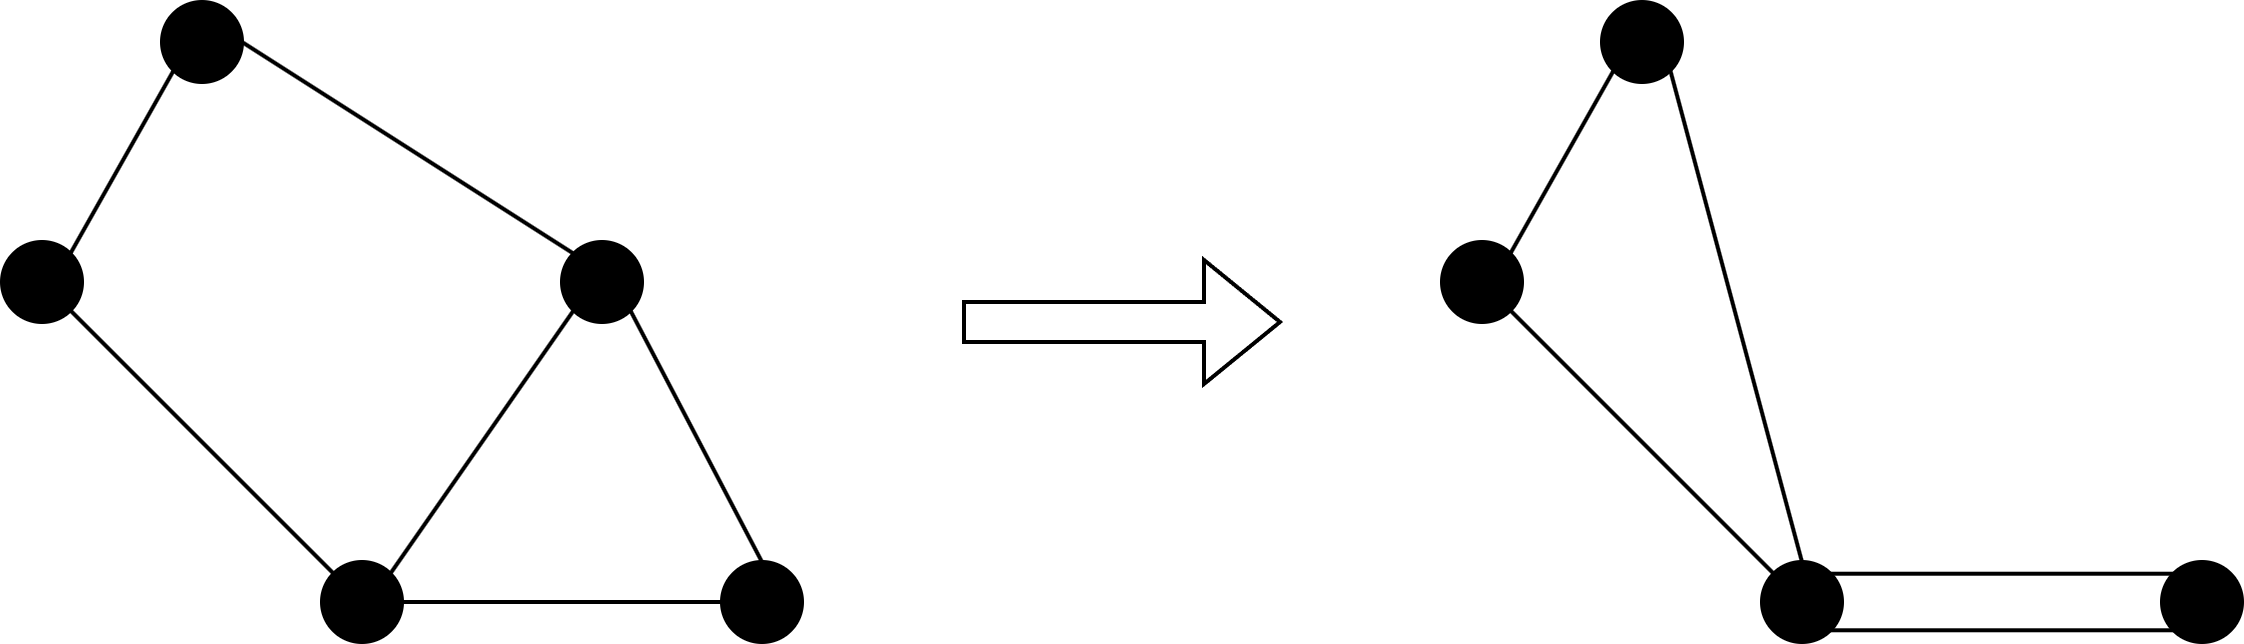
\includegraphics[width=0.8\linewidth]{images/ed.png}
    \caption{Edge contraction}
\end{figure}
Let $G=(V,E)$ be a multigraph without self-loops, and let $e=\{u,v\}\in E$. 
Formally, the contraction of $e$, denoted $G\setminus e$, is formed by:
\begin{enumerate}
    \item Replacing vertices $u$ and $v$ with a new vertex $w$.
    \item Replacing all edges $(u,x)$ or $(v,x)$ with an edge $(w,x)$.
    \item Removing any self-loops involving $w$.
\end{enumerate}
After contraction, the graph $G\setminus e$ is still a multigraph. 
A crucial observation is that contracting an edge $(u,v)$ preserves cuts where both $u$ and $v$ belong either to the same set $S$ or to its complement $S^\prime$.
For a cut $\delta(S)$ in the original graph $G$, if $u,v\in S$, then after contraction, $\delta_G(S)=\delta_{G\setminus e}(S)$, where $w$ is substituted for $u$ and $v$.

\paragraph*{Algorithm}
Karger's algorithm for finding a minimum cut works as follows:
\begin{enumerate}
    \item Pick an edge uniformly at random and contract the two vertices at its endpoints.
    \item Repeat the contraction process until only two vertices remain (i.e., after $n-2$ edges have been contracted).
\end{enumerate}
The two remaining vertices represent a partition $(S, S^\prime)$ of the original graph, and the edges between them correspond to the cut $\delta$(S) in the input graph.

Let $k$ be the size of the minimum cut. 
Focus on a particular minimum cut $\delta(S)$ where $|\delta(S)|=k$
\begin{lemma}
    Let $\delta(S)$ be a minimum cut in the graph $G=(V,E)$. 
    The probability that Karger's algorithm outputs the cut $\delta(S)$ is at least:
    \[\Pr(\text{Karger's algorithm ends with the cut }\delta(S))\geq\dfrac{1}{\binom{n}{2}}\]
\end{lemma}
\begin{proof}
    Let the contracted edges be $\left\{e_1,e_2,\dots,e_{n-2}\right\}$. 
    The algorithm succeeds if none of the contracted edges are part of the minimum cut $\delta(S)$.

    Initially, the input graph $G$ has at least $\frac{nk}{2}$ edges, since the minimum degree in $G$ is at least $k$. 
    Otherwise, we could disconnect a vertex with fewer than $k$ edges, forming a smaller cut, which contradicts the assumption that $\delta(S)$ is a minimum cut.

    After $j$ contractions, the multigraph $G_j$ contains $n - j$ vertices, and its minimum degree is still at least $k$. 
    Thus, $G_j$ has at least $\frac{(n - j)k}{2}$ edges.

    The probability that the algorithm successfully finds the minimum cut $\delta(S)$ is the probability that none of the contracted edges belong to $\delta(S)$. 
    This probability is bounded below by:
    \begin{align*}
        \Pr(\text{final graph} = \delta(S)) &= \Pr(e_1, e_2, \dots, e_{n-2} \notin \delta(S)) \\
                                            &= \Pr(e_1 \notin \delta(S)) \prod_{j=1}^{n-3} \Pr(e_{j+1} \notin \delta(S) \mid e_1, \dots, e_j \notin \delta(S)) \\
                                            &\geq \prod_{j=0}^{n-3} \left( 1 - \frac{k}{(n-j)k/2} \right) \\
                                            &= \frac{n-2}{n} \times \frac{n-3}{n-1} \times \cdots \times \frac{2}{4} \times \frac{1}{3} \\
                                            &= \frac{2}{n(n-1)} \\
                                            &= \frac{1}{\binom{n}{2}}
    \end{align*}
\end{proof}
To increase the probability of success, we run the algorithm $l\cdot \binom{n}{2}$ times. 
The probability that at least one run succeeds is:
\[\Pr(\text{one success})=1-\left(1-\dfrac{1}{\binom{n}{2}}\right)^{l\cdot\binom{n}{2}}\geq 1-e^l\]
By setting $l = c \log n$, the error probability becomes $\frac{1}{n^c}$. 

\paragraph*{Complexity}
One run of Karger's algorithm takes $\mathcal{O}(n^2)$ time.
Hence, by repeating the algorithm $\mathcal{O}(n^2\log n)$ times, we obtain a randomized algorithm with total time complexity $\mathcal{O}(n^4\log n)$ and an error probability of at most $\frac{1}{\text{poly}(n)}$.

\subsection{Karger and Stein algorithm}
Karger and Stein introduced a more efficient version of Karger's original algorithm by refining its edge contraction process.
The key insight comes from analyzing the telescoping product that emerges when calculating the probability of contracting an edge from the minimum cut set $\delta(S)$. 

In the early stages of the contraction, it is very unlikely that an edge from the minimum cut is contracted. 
However, as the graph shrinks, the likelihood of contracting such an edge increases. 
The probability that a fixed minimum cut $\delta(S)$ survives down to a smaller subgraph with $l$ vertices is at least:
\[\Pr(\text{cut survives})=\frac{\binom{l}{2}}{\binom{n}{2}}\]
By choosing $l=\frac{n}{\sqrt{2}}$, we ensure that the probability of retaining the minimum cut is at least $\frac{1}{2}$.
This means that, in expectation, two trials of the algorithm should suffice to find the minimum cut with high probability.

\paragraph*{Algorithm}
The steps of Karger and Stein algorithm are: 
\begin{enumerate}
    \item From a multigraph $G$ with at least six vertices, repeat the following twice: 
        \begin{enumerate}
            \item Run the original edge contraction algorithm until the graph is reduced to $\frac{n}{\sqrt{2}}+1$ vertices.
            \item Recur on the resulting contracted graph.
        \end{enumerate}
    \item Return the minimum of the cuts found in the two recursive calls.
\end{enumerate}
The choice of six as the threshold for recursion depth does not impact the overall asymptotic complexity, but only affects the running time by a constant factor.
\begin{algorithm}[H]
    \caption{Karger and Stein}
    \begin{algorithmic}[1]
        \Function{contract}{$G=(V,E), t$}
            \While{$|V| > t$}
                \State Choose $e\notin E$ uniformly at random
                \State $G=G\setminus e$
            \EndWhile 
            \State \Return $G$
        \EndFunction
        \Statex
        \Function{fastmincut}{$G= (V,E)$}
            \If {$|V| < 6$}
                \State \Return mincut($V$)
            \Else 
                \State $t= \left\lceil  1 + \frac{|V|}{\sqrt{2}}\right\rceil$
                \State $G_1 =$ \Call{contract}{$G, t$}
                \State $G_2 =$ \Call{contract}{$G, t$}
                \State \Return $\min \{$\Call{fastmincut}{$G_1$}, \Call{fastmincut}{$G_2$}$\}$
            \EndIf
        \EndFunction
    \end{algorithmic}
\end{algorithm}  

\paragraph*{Complexity}
The recurrence relation for the running time of the Karger-Stein algorithm is:
\[T(n) = 2n^2 + T\left(\frac{n}{\sqrt{2}}\right)\]
Which solves to:
\[T(n) = \mathcal{O}(n^2 \log n)\]
The algorithm succeeds with probability at least $\geq \frac{1}{2}$ at each recursive step. 
To boost the probability of success, we repeat the algorithm multiple times. 
Specifically, the recurrence for the success probability $\Pr(n)$ is: 
\[\Pr(n) \geq 1 - \left( 1 - \frac{1}{2}\Pr\left(\frac{n}{\sqrt{2}} + 1\right)\right)^2\]
This implies that:
\[\Pr(n) = \Omega\left(\frac{1}{\log n}\right)\]
To ensure the algorithm succeeds with high probability we need to run the algorithm $\mathcal{O}(\log^2 n)$ times. 
Thus, the total time complexity of the Karger-Stein algorithm is: 
\[\mathcal{O}(n^2 \log^3 n)\]
\begin{corollary}
    Any graph has at most $\mathcal{O}(n^2)$ distinct minimum cuts.
\end{corollary}
Like the original Karger's algorithm, the Karger-Stein algorithm is a Monte Carlo algorithm. 
This means that it guarantees a correct solution with high probability, but there remains a small probability of failure.